\thispagestyle{lichsutoanhocnone}
\pagestyle{lichsutoanhoc}
\graphicspath{{../lichsutoanhoc/pic/}}
\everymath{\color{lichsutoanhoc}}
\blfootnote{$^*$\color{lichsutoanhoc}Bài viết của Eva Kaufholz--Soldat về những điểm kết nối một nhà toán học, một hoạ sĩ và một nhà văn.}
\begingroup
\AddToShipoutPicture*{\put(0,616){\includegraphics[width=19.3cm]{../bannerlichsu}}}
\AddToShipoutPicture*{\put(80,525){\includegraphics[scale=1]{../tieude.pdf}}}
\centering
\endgroup

\vspace*{183pt}

\begin{multicols}{2}
	\textit{\textbf{\color{lichsutoanhoc}Lời người dịch:}} Nhắc tới nhà toán học nữ Kovalevskaya, người ta hay miêu tả một cuộc đời khổ đau và bất hạnh, bên cạnh những vinh quang khoa học. Vào năm $1976$, cuốn tiểu thuyết về Kovalevskaya -- \textit{Một số phận vinh quang và cay đắng} -- của tác giả Lyubov Vorolsova cũng đã được giới thiệu với các độc giả ở Việt Nam. Tuy nhiên, có phải thực sự số phận của Kovalevskaya chỉ toàn vị đắng mà không có những tia nắng ấm áp? Cũng cần nhắc lại rằng, bên cạnh những thành tích vẻ vang trong khoa học, Sofia Kovalevskaya còn là một nhà văn và nhà biên kịch. Trong những năm tháng cuối đời bà quay lại với công việc viết văn từng say mê từ thời niên thiếu thông qua việc viết những dòng hồi ức, soạn kịch bản. Tại Stockholm, có một thời gian Sofia sống tại nhà của Mittag--Leffler và có một tình bạn gắn bó với em gái của nhà toán học là Anna Leffler. Chính Anna đã động viên Sofia trau dồi thêm kỹ năng viết văn, và họ đã cùng sáng tác một số vở kịch, trong đó có một vở mang tên \textit{Đấu tranh với Hạnh phúc}. Sofia cũng đã viết các cuốn hồi ký về tuổi thơ của mình ở nước Nga và  một cuốn tiểu thuyết bán tự truyện mang tên \textit{Cô gái Hư vô}.  Trong một cuốn hồi ký được xuất bản sau khi bà qua đời, Kovalevskaya viết ``\textit{Không thể là một nhà toán học mà không phải là một nhà thơ trong tâm hồn}". Trong bài viết này, tác giả Eva Kaufholz--Soldat giúp chúng ta phần nào hiểu rõ hơn về nguồn gốc ra đời những chủ điểm vốn được mặc định gán cho cuộc đời của nhà toán học nữ tài ba, bao gồm cả sự bất hạnh và vẻ ngoài không hấp dẫn của Sofia Kovalevskaya.
	\vskip 0.1cm
	Một bài báo cũ trích từ \textit{The Daily Chronicle} (London), ngày $6$ tháng $5$ năm $1901$, cho thấy một bức tranh phản ánh nguồn gốc lịch sử của các định kiến xã hội về những phụ nữ nổi tiếng trong các lĩnh vực sáng tạo do nam giới thống trị. 
	\begin{figure}[H]
		\vspace*{-5pt}
		\centering
		\captionsetup{labelformat= empty, justification=centering}
		\includegraphics[width= 0.8\linewidth]{1}
%		\caption{\small\textit{\color{}}}
		\vspace*{-5pt}
	\end{figure}
	``\textit{Có thể một số phụ nữ với tài năng không thể tranh cãi đã phải chịu đựng những nỗi đau tương tự. Ngài George Smith đã để ghi lại một ấn tượng rằng Charlotte Brontë sẽ từ bỏ tất cả danh tiếng của mình để đổi lại sắc đẹp. Điều này đã phủ một ánh sáng đáng thương hại lên con người của Jane Eyre. Jane có nhan sắc bình thường, nhưng là một sự bình thường khiến Rochester mê mẩn. Người tạo ra cả hai nhân vật có bao giờ tự hỏi mình liệu vẻ ngoài của chính cô  có thể chế ngự được sự quyến rũ nữ tính hoang dã đó  hay không? Sonia Kovalevsky [Sofia Kovalevskaya] không xinh đẹp, và sự nổi tiếng khắp châu Âu về tài năng toán học của bà không thể xoa dịu một trái tim đầy những đam mê không được đáp lại. Trong một giai đoạn phát triển nào đó trong tương lai, những người phụ nữ có thể thực sự ``bình tĩnh như một quyền lực, và thờ ơ như một tinh thần cao thượng"; nhưng thời điểm đó dường như vẫn còn xa vời. Marie Bashkirtseff nói một cách khôn ngoan rằng tình yêu không dành cho người nghệ sĩ, ngoại trừ như một thứ xa xỉ mà anh ta có thể trả tiền để có được, `khi anh ta đã giành được vị trí của mình'}."
	\begin{figure}[H]
		\vspace*{-5pt}
		\centering
		\captionsetup{labelformat= empty, justification=centering}
		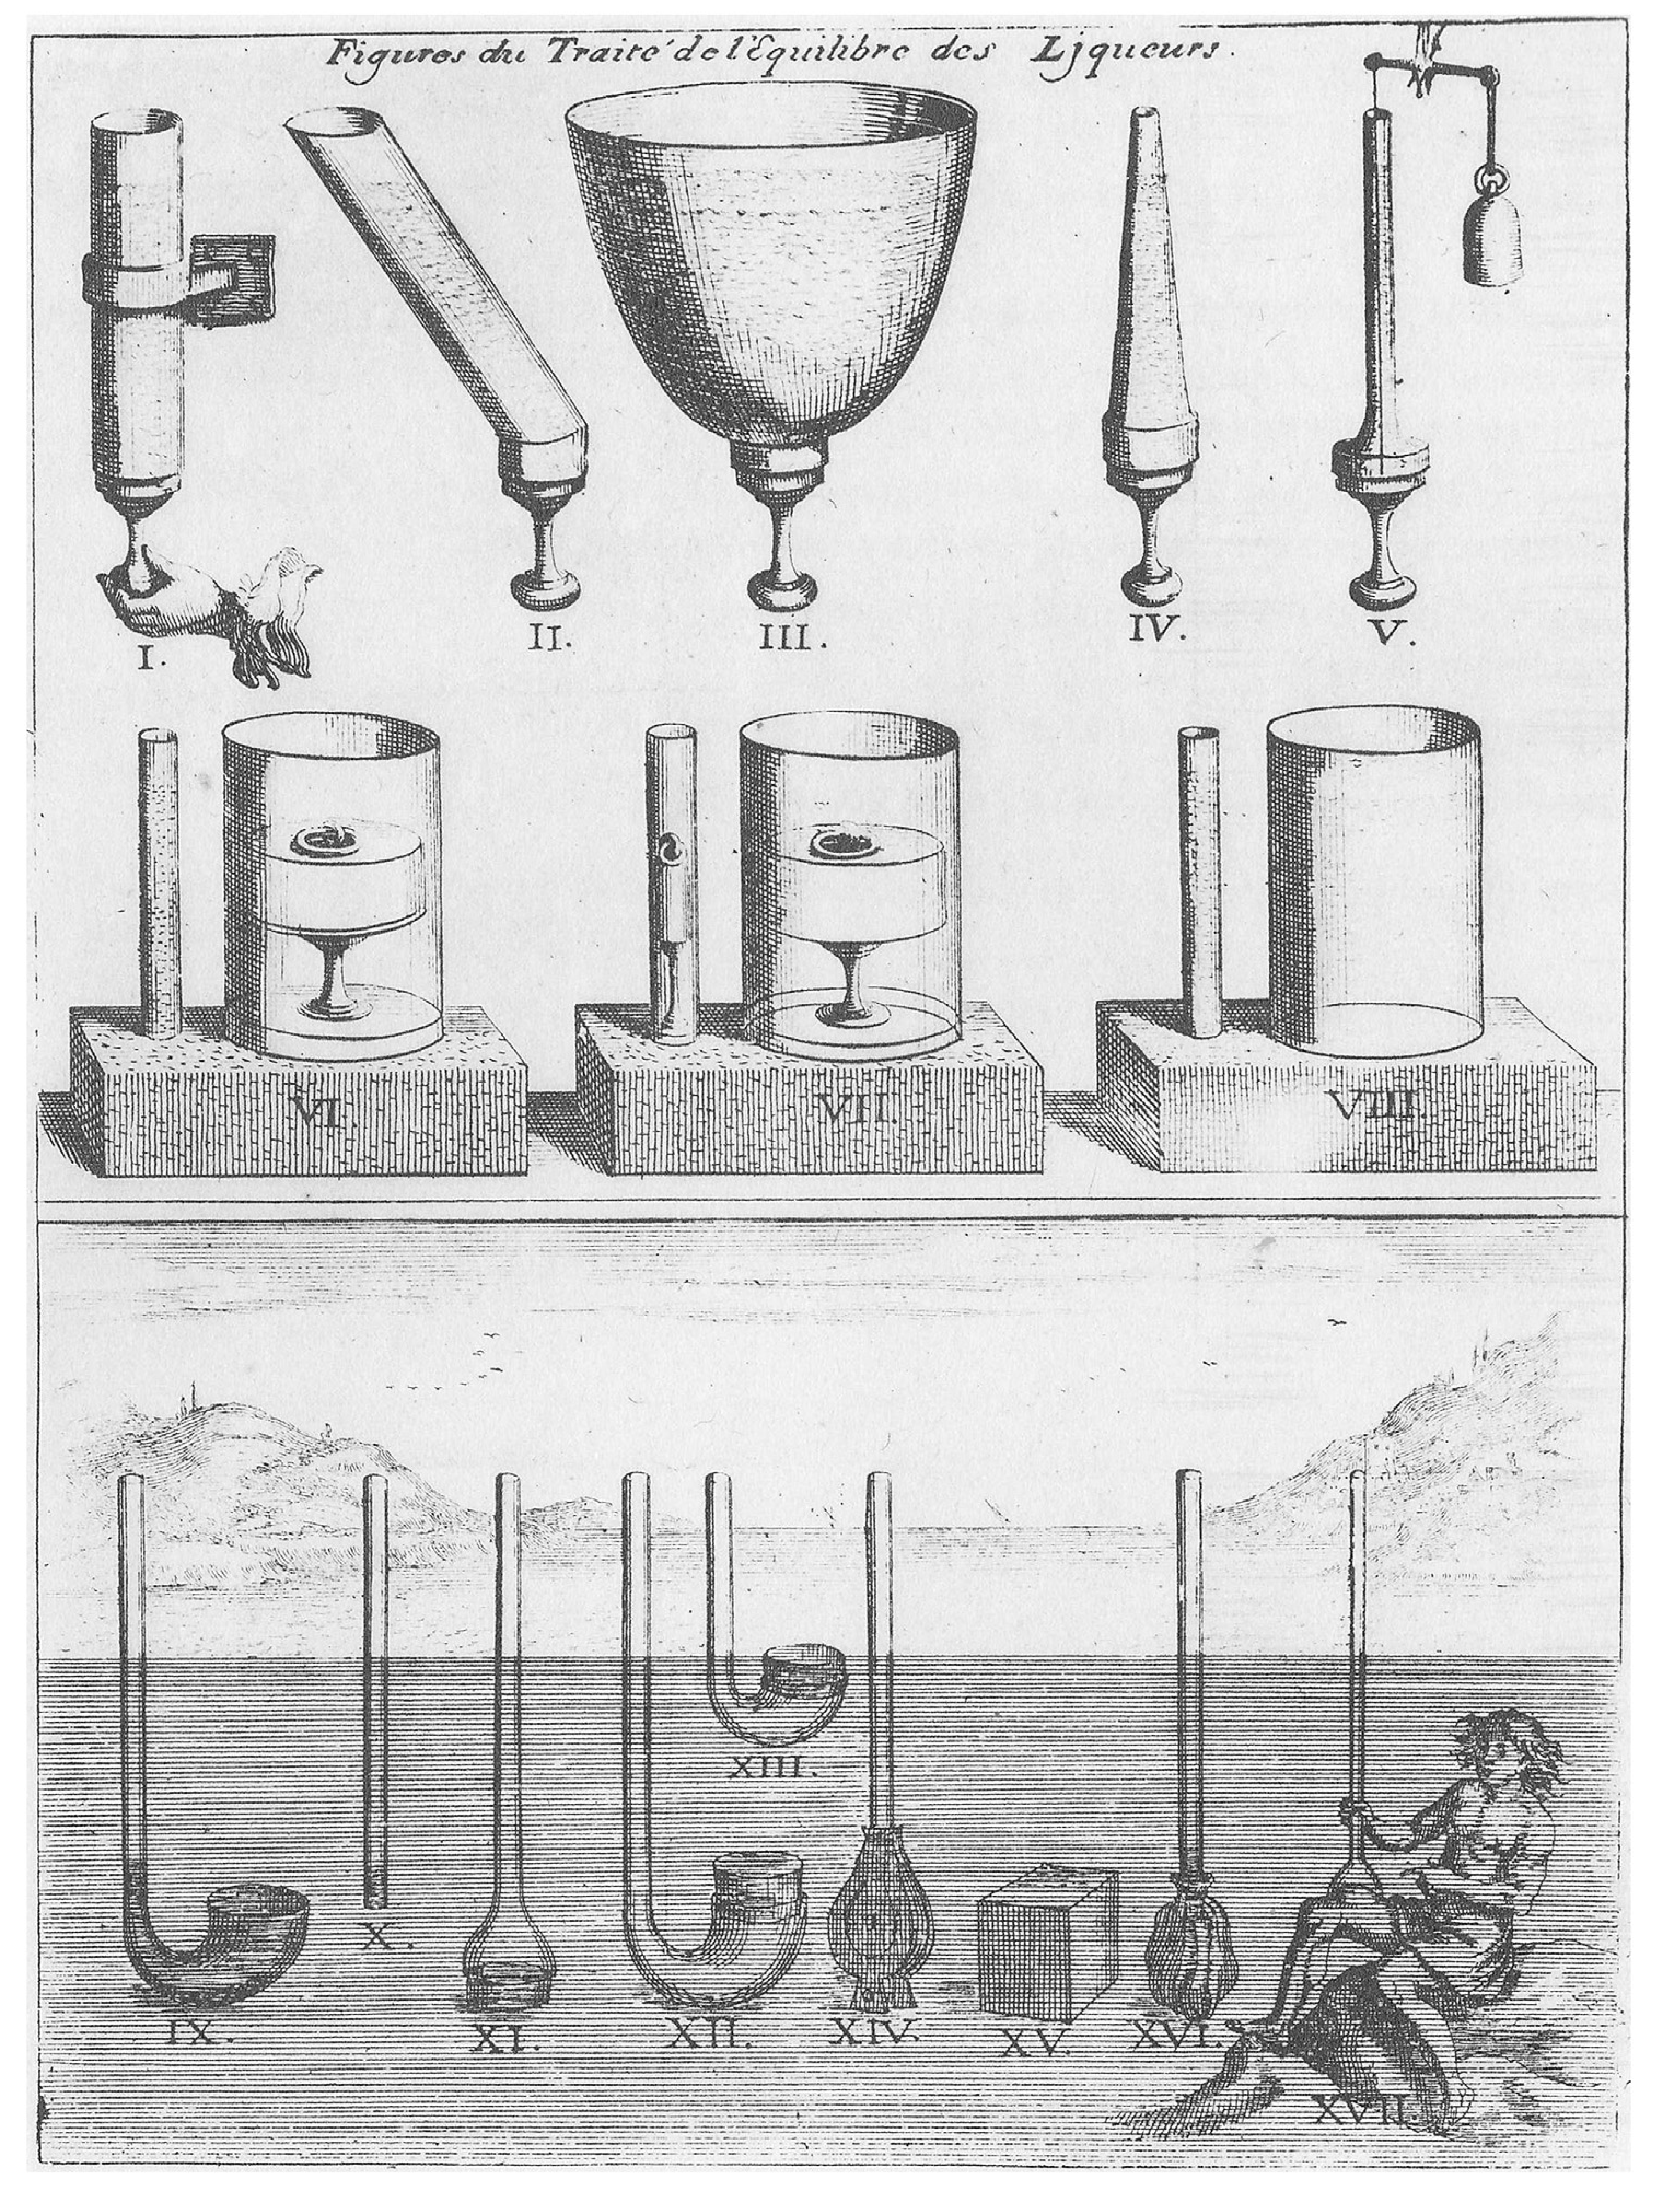
\includegraphics[width= 0.75\linewidth]{2}
		\caption{\small\textit{\color{lichsutoanhoc}Charlotte Brontë.}}
		\vspace*{-10pt}
	\end{figure}
	Tên của ba người phụ nữ được nhắc đến là: Marie Bashkirtseff $(1858-1884)$, người đạt tới danh vọng của một họa sĩ sau khi được đào tạo tại Académie Julian ở Paris; Charlotte Brontë $(1816-1855)$, tác giả nổi tiếng với Jane Eyre; và Sofia Kovalevskaya $(1850-1891)$, một trong những nhà toán học lừng danh. Đây là những người phụ nữ phi thường, có vị trí trong thế giới nghệ thuật hoặc toán học, những lĩnh vực được coi là do nam giới thống trị vào đầu thế kỷ $19$ và $20$. Ông George Smith được nhắc tới là nhà biên tập khắt khe của nữ văn sỹ Brontë.
	\begin{figure}[H]
		\vspace*{-5pt}
		\centering
		\captionsetup{labelformat= empty, justification=centering}
		\includegraphics[width= 0.75\linewidth]{3}
		\caption{\small\textit{\color{lichsutoanhoc}Marie Bashkirtseff.}}
		\vspace*{-10pt}
	\end{figure}
	Tất cả chúng ta chắc cũng đã biết tới một loại ấn phẩm có thể được gọi là ``bảng liệt kê bách khoa toàn thư", dạng ấn phẩm liệt kê tên của những người phụ nữ xuất sắc trong khoa học hoặc nghệ thuật  nhằm vào nhóm độc giả trẻ tuổi, thông qua tường thuật về những cuộc đời phi thường này để khuyến khích độc giả, đặc biệt là các em gái, theo đuổi sự nghiệp trong các ngành khoa học và công nghệ. Các ấn phẩm dạng bách khoa như vậy cũng được xuất bản thường xuyên vào đầu thế kỷ $20$, đặc biệt là trên báo chí hoặc trong các công trình thảo luận về phụ nữ và vai trò của họ trong xã hội. Bài báo nổi bật được trích dẫn ở trên đây là một ví dụ. Nhưng giọng văn của đoạn báo được trình bày ở đây dường như không hợp với các câu chuyện tiểu sử về những người phụ nữ phi thường làm hình mẫu cho các cô gái trẻ. Kovalevskaya, Bashkirtseff và Brontë trên thực tế không hề được miêu tả theo cách tích cực trong đoạn trích này. Nó nói nhiều hơn về sự đau khổ của họ (``cơn đau"), nỗi đau của họ (ở đây theo nghĩa tâm lý), trước khi thảo luận chi tiết về vóc dáng bề ngoài có vẻ kém hấp dẫn của họ.
	\begin{figure}[H]
		\vspace*{-5pt}
		\centering
		\captionsetup{labelformat= empty, justification=centering}
		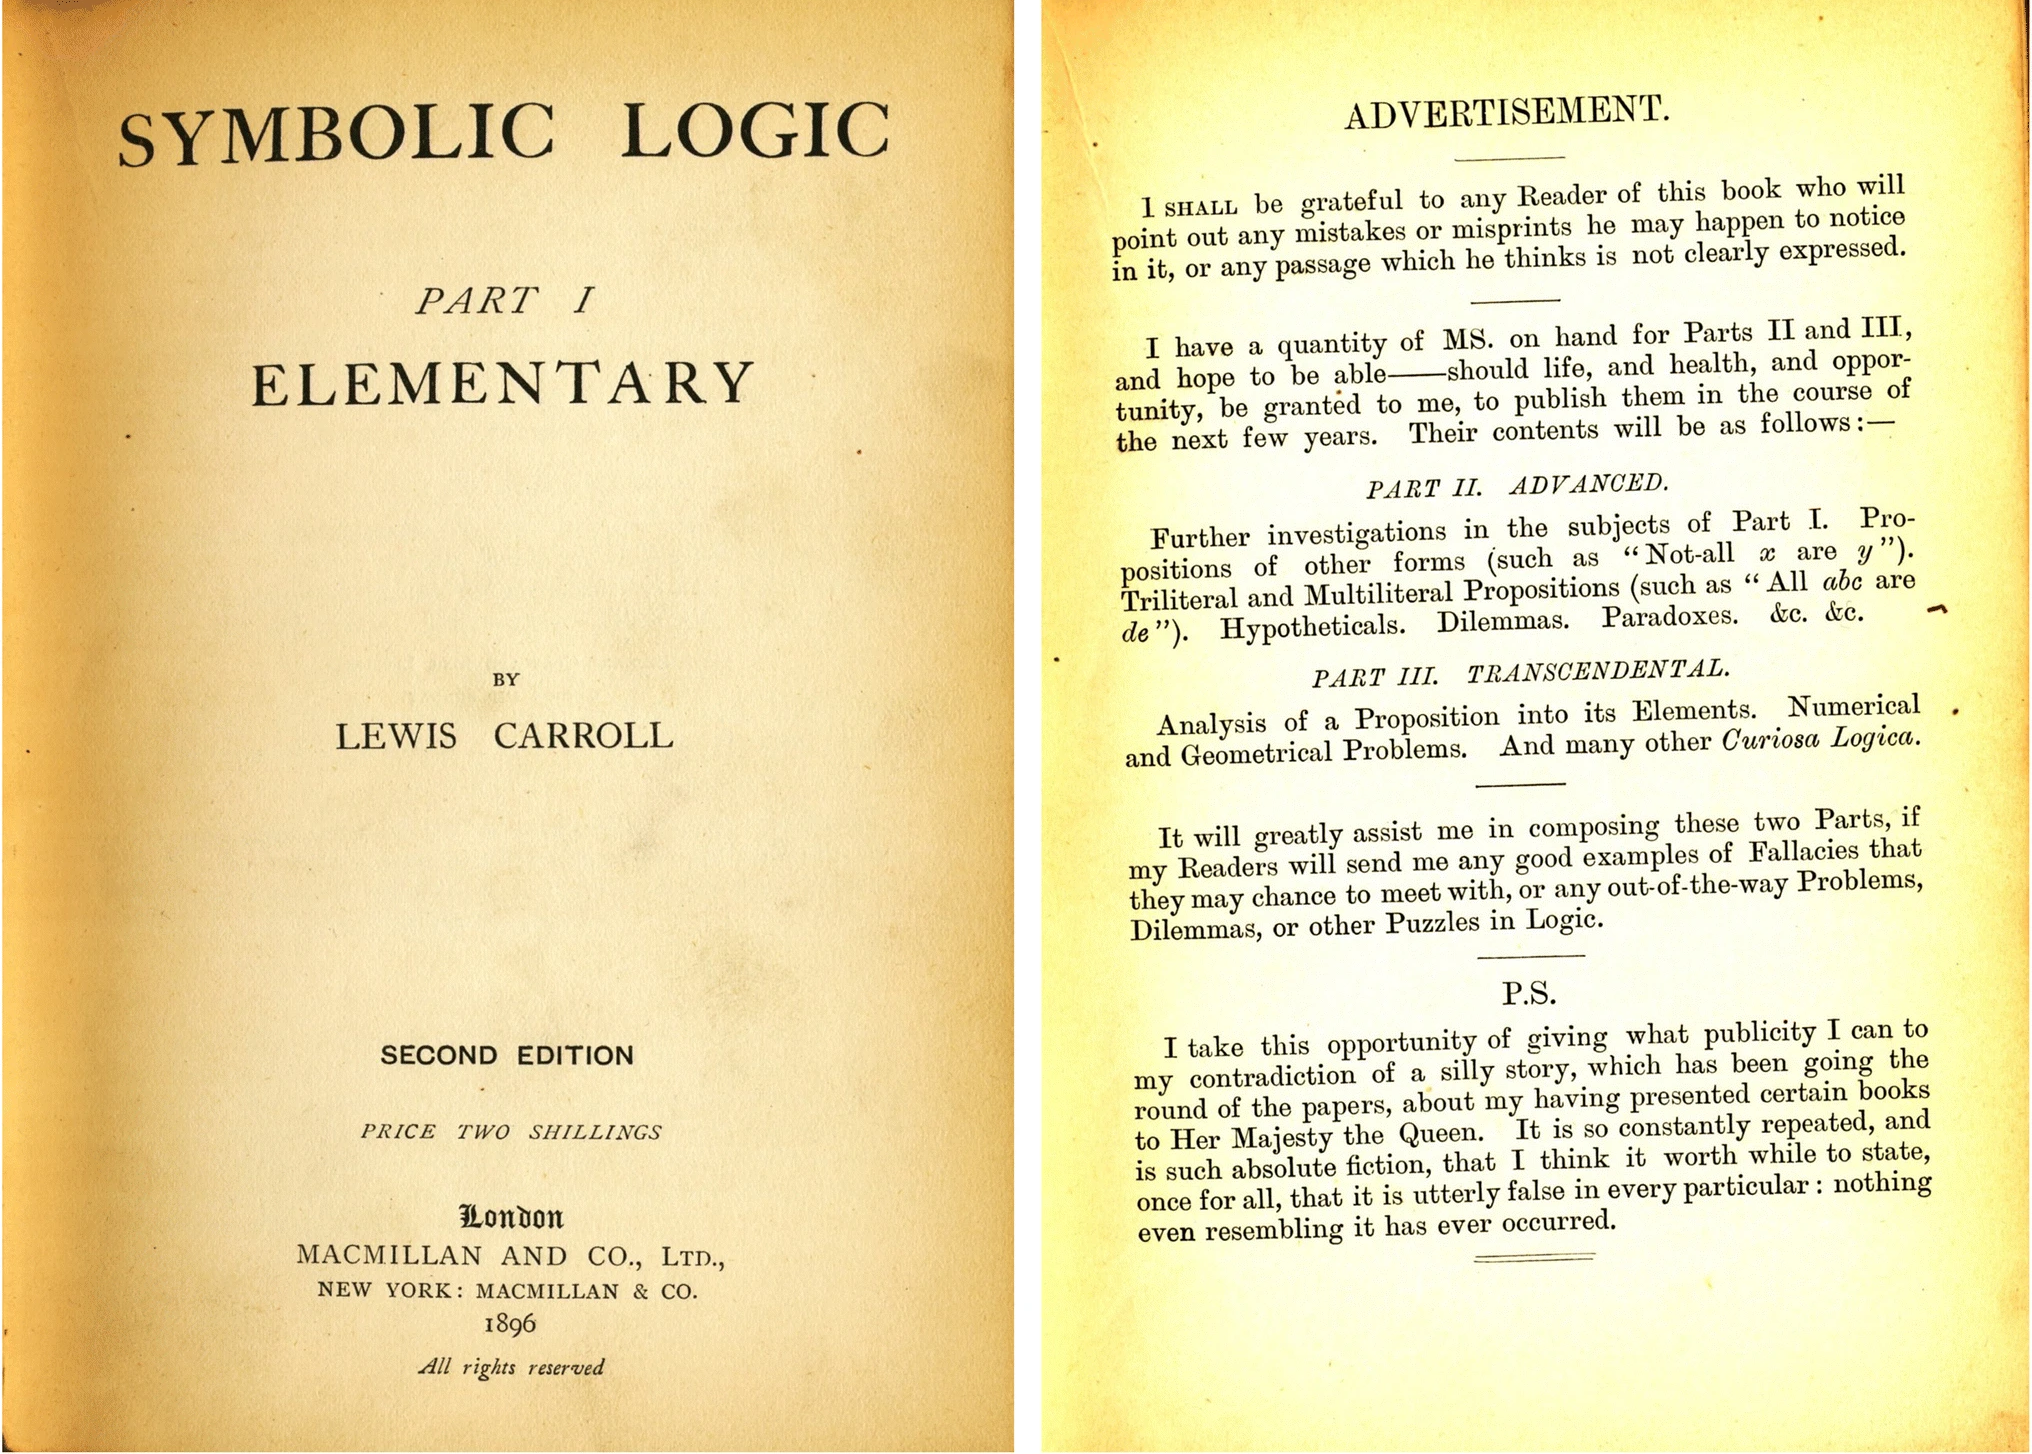
\includegraphics[width= 0.75\linewidth]{4}
		\caption{\small\textit{\color{lichsutoanhoc}Sofia Kovalevskaya.}}
		\vspace*{-10pt}
	\end{figure}
	Đoạn trích trên nhằm cảnh báo các cô gái trẻ không nên đi theo vết chân của Kovalevskaya, Bashkirtseff và Brontë, ba người phụ nữ thường được nhắc đến nhiều nhất trong các cuộc tranh luận với những dụng ý trái ngược nhau.  Những người phụ nữ này thực sự được liên kết với nhau bởi nhiều thứ khác ngoài nghề nghiệp vốn đặc biệt của họ vào thời điểm đó. Vào thời điểm bài báo năm $1901$ xuất hiện, cả ba người đều đã qua đời khi còn khá trẻ. Brontë qua đời năm $1855$ ở tuổi $38$, có thể là do biến chứng khi mang thai, Bashkirtseff qua đời vì bệnh lao năm $1884$ ở tuổi $25$, trong khi Kovalevskaya chết vì nhiễm trùng phổi sau sinh nhật lần thứ $41$ vào năm $1891$. Một số bài báo ra mắt sau khi họ qua đời đã viết về mỗi người trong số họ, và khác xa với việc mô tả họ là những  người phụ nữ tiên phong và thành đạt, các bài báo đó lại trình bày họ như những minh chứng áp đặt chỉ ra sự thất bại không thể tránh khỏi của những người phụ nữ mưu cầu tới một sự nghiệp khác ngoài vai trò làm vợ và làm mẹ.
	\vskip 0.1cm
	``\textit{Tình yêu viên mãn là mục tiêu thực sự trong cuộc đời người phụ nữ}". Câu  nói này có nguồn gốc từ  cuốn tiểu sử về Kovalevskaya của tác giả Anna Charlotte Leffler ($1849-1892$),  em gái của Gösta Mittag--Leffler và là bạn thân của nhà toán học nữ, và cũng là một tác giả nổi tiếng trên văn đàn quốc tế. Như phụ đề của cuốn sách -- \textit{Những gì tôi học được với cô ấy và những gì cô ấy nói với tôi về bản thân} -- đã chỉ ra, bài thuật được viết vào năm $1892$ của Anna Leffler dựa trên những kinh nghiệm được chia sẻ, những câu chuyện do Kovalevskaya kể cũng như những đoạn trích từ thư từ được trích dẫn trực tiếp. Tất nhiên, điều này không có nghĩa đây là một bài thuật khách quan. Bản thân Leffler đã mô tả cuốn tiểu sử của mình như một ``bài thơ". Ta không khó để nhận ra rằng Anna, một mặt đã sử dụng những giai thoại và trích dẫn có chủ đích, nhưng mặt khác cũng đưa vào đánh giá cá nhân thường được bộc lộ một cách cởi mở của chính bà, đã hoàn toàn không muốn viết ra một cuốn chân dung của một người phụ nữ chiến thắng trong một lĩnh vực dành cho nam giới. Dựa trên kinh nghiệm của bản thân, Leffler giải thích rằng tình yêu viên mãn là mục tiêu tối cao trong cuộc sống của phụ nữ và chẩn đoán rằng đây chính là điều mà Kovalevskaya chưa bao giờ đạt được, mặc dù đó là mong muốn lớn nhất của cô. Vì vậy, Leffler giới thiệu cuộc sống của người bạn thân của mình như là cuộc sống của  một người phụ nữ chịu thất bại, bị giằng xé giữa khát khao của trái tim và nghề nghiệp lựa chọn của mình, và vì lý do này mà cuối cùng cô ấy đã chết.
	\vskip 0.1cm
	Chính tại đây đã bắt nguồn truyền thuyết về một Kovalevskaya bất hạnh, một mô--típ thậm chí còn trở nên được phổ biến hơn bởi \textit{Cuốn sách về phụ nữ} của Laura Marholm vào năm $1894$, một tác phẩm mà thành công của nó có lẽ cũng là do tính chất gây tranh cãi của nó đem tới. Mặc dù chưa bao giờ gặp nhà toán học, Marholm tin chắc rằng bà đã hiểu rõ bản chất của phụ nữ đến mức chỉ có mình mới biết lời giải thích thực sự cho sự bất hạnh của Kovalevskaya. Theo Marholm, chính trí thông minh vượt trội của Kovalevskaya đã ngăn cản cô tìm được một người đàn ông có khả năng trao cho cô tình yêu chân thành mà cô hằng mong ước. Laura Marholm là người chú trọng nhất đến ngoại hình của Kovalevskaya. Ví dụ, theo nhu cầu phân loại rộng rãi vào thời điểm đó, phụ nữ Nga được chia ra thành hai loại. Theo Marholm, một mặt, có những phụ nữ gợi cảm và nữ tính, đó cũng là những người có nhiều phẩm chất lôi cuốn người khác giới. Nhóm còn lại, trong đó Laura liệt kê ra Kovalevskaya, thì hoàn toàn ngược lại. Marholm vẽ nên bức tranh về những người phụ nữ sở hữu những thuộc tính nam giới -- những đặc điểm thường được huy động trong lý thuyết về tính cách giới tính: họ rõ ràng, can đảm, mạnh mẽ và ``biết lý lẽ". Nhưng điều này cũng được phản ánh trong vẻ ngoài của họ, không được nữ tính cho lắm: ``\textit{Có một cái gì đó trung lập về họ; có thể nói là người ta không nhận thức được rằng họ là phụ nữ}" [$5$~tr.~$168$]. Nói tóm lại, một quý cô có thể suy nghĩ như đàn ông thì không thể trông giống một phụ nữ.
	\vskip 0.1cm
	Sau Marholm, trong một thời gian dài không có ấn phẩm nào xuất hiện trong đó vẻ ngoài của Kovalevskaya được trình bày một cách tích cực. Tuy nhiên, trong khi sự xấu xí được gán cho Brontë (mặc dù thực tế là hầu như không có bức chân dung nào về nữ văn sỹ được kiểm chứng) đã được thảo luận lại nhiều lần trong các tài liệu gần đây [$3$~tr.~$55-59$],  có một bước ngoặt hoàn toàn trong việc đánh giá cao nhà toán học nữ diễn ra từ những năm $1930$. Nó có lẽ bắt nguồn từ một cáo phó viết vào năm $1935$ bởi Hermann Weyl ($1885-1955$) về đồng nghiệp của ông là Emmy Noether ($1882-1935$). Weyl nâng Kovalevskaya lên hàng ngũ hiện thân của nữ tính, cả về hình thức bên ngoài và liên quan đến các thuộc tính tính cách về giới tính vẫn còn thịnh hành lúc đó. Weyl lưu ý rằng Kovalevskaya không chỉ sở hữu ``vẻ quyến rũ nữ tính" mà còn có ``nhân cách hoàn thiện nhất", ``một nhân cách của một người phụ nữ", trong đó bao gồm cả khía cạnh  cảm xúc mà Noether còn thiếu: ``Với [Kovalevskaya], bạn thấy sự căng thẳng giữa tâm trí sáng tạo của cô ấy, cuộc sống và niềm đam mê của cô ấy, và tinh thần tự chế giễu bản thân một cách mỉa mai trước cuộc xung đột tuyệt vọng của chính cô. Điều này là quá xa vời đối với khả năng của Emmy!" Do đó, Kovalevskaya là một phản đề của Noether, người mà Weyl đã mô tả là trông nam tính. Noether đã được giới thiệu là một nhà toán học giỏi hơn, nhưng Weyl nói về bà đúng như những gì Ellen Key, một nhà sư phạm danh tiếng đã nói về Kovalevskaya khoảng ba mươi năm trước: ``Không ai có thể nói rằng Ân Huệ đã đứng gần cái nôi của bà (lúc mới chào đời)" [$6$~tr.~$219$]. Chắc chắn không phải ngẫu nhiên mà Eric Temple Bell ($1883-1960$) đã mô tả Kovalevskaya là ``xinh đẹp" và nói về một ``phụ nữ trẻ rực rỡ" trong tác phẩm có tựa đề hoàn toàn không phù hợp \textit{Những người đàn ông của Toán học} xuất bản hai năm sau đó [$1$~tr.~$424$]. Tuy nhiên, thậm chí ngay cả ngày nay, Kovalevskaya không chỉ được mô tả là xinh đẹp mà thậm chí còn được coi là ``chắc chắn là nhà toán học xinh đẹp nhất của cả hai giới tính" [$2$~tr.~$78$].
	\vskip 0.1cm
	Theo cách thể hiện hiện đại, Kovalevskaya không đơn thuần là một hình mẫu. Bà thường được đặt trên bục tượng đài cao vời vợi, không nhất thiết theo một cách có ý thức, và được thể hiện như một nhân vật mang tính biểu tượng, người phải bác bỏ mọi định kiến về các nhà khoa học nữ. Do đó, điều này không chỉ được coi là bằng chứng cho thấy phụ nữ có khả năng đạt được những thành tích cao nhất trong toán học, mà còn chứng minh rằng họ không nhất thiết phải có ngoại hình xấu xí thì mới quan tâm đến nghiên cứu. Kovalevskaya, cũng như Bashkirtseff và Brontë, ngày nay được tôn sùng như những người tiên phong và những nữ anh hùng, là những người phụ nữ mà nhờ những thành tích đặc biệt của họ đã có thể thành công trong các lĩnh vực hầu như chỉ dành cho nam giới như toán học, hội họa hoặc văn học. Không ai còn có thể nghĩ đến việc quy kết cái chết sớm của họ cho bất cứ điều gì khác ngoài việc chăm sóc y tế không đạt tiêu chuẩn, hoặc coi sự lựa chọn nghề nghiệp của họ là nguồn gốc của một cuộc sống dành cho đam mê bị chối bỏ.
	\vskip 0.1cm
	Và cũng do vậy, Bashkirtseff, Brontë và Kovalevskaya đã trở thành những tấm vải vẽ, trên đó các tác giả khác nhau đã phóng chiếu  những luận đề tương ứng của họ về vị trí của phụ nữ trong khoa học và nghệ thuật, như đã từng diễn ra hồi đầu thế kỷ $20$. Mặc dù, tất nhiên, không nên quên rằng ngày nay chắc chắn có nhiều bức chân dung đa dạng hơn về ba người phụ nữ phi thường này, thì cũng có nhiều người theo đuổi một mục đích được vạch ra rõ ràng, điều này đặc biệt đúng đối với các dạng ấn phẩm liệt kê bách khoa toàn thư hiện đại đã được đề cập ở trên. Mục đích đằng sau hình thức phóng chiếu thể hiện này, cụ thể là trình bày những tiểu sử chi tiết hơn của những người phụ nữ phi thường  làm hình mẫu cho các học sinh nữ noi theo, chắc chắn là đáng khen ngợi từ quan điểm hiện đại. Nhưng có một số yếu tố chỉ ra rằng hành động này có thể có phản tác dụng:
	\vskip 0.1cm
	Huyền thoại và lối hùng biện làm suy yếu khoa học và, theo tôi, khiến cho nó xa lánh những người trẻ tuổi (và đặc biệt là các học sinh nữ): chúng tạo ra niềm tin ít nhiều có ý thức rằng phụ nữ hoặc các em gái phải đặc biệt tốt và anh hùng mới có thể cống hiến hết mình cho khoa học hoặc toán học. (xem [$4$~tr.~$309$]).
	\vskip 0.1cm
	Điều này không có nghĩa là kể từ bây giờ những người phụ nữ trẻ nên tránh xa những cuốn tiểu sử kiểu tụng ca như vậy. Tuy nhiên, cần phải kết hợp cách tiếp cận này với một cuộc thảo luận về những định kiến mới đã nảy sinh, đồng thời trình bày các mô hình thực tế hơn, để các phụ nữ trẻ thấy được những điều kiện tiên quyết thực sự và các cơ hội nghề nghiệp khác nhau trong toán học là gì, và do đó có được sự nhiệt tình về môn học này.
	\vskip 0.1cm
	\textbf{\color{lichsutoanhoc}Về tác giả:} Eva Kaufholz--Soldat học Toán và Lịch sử Khoa học tại Đại học Hamburg. Sau khi lấy được bằng tiến sĩ từ Đại học Johannes Gutenberg Mainz, cô hiện vừa là giám đốc Trung tâm viết về Khoa học Tự nhiên và Toán học, vừa là nhà nghiên cứu, tập trung vào những người phụ nữ trong toán học vào thời điểm chuyển giao sang thế kỷ $20$, tại Đại học Goethe, Frankfurt. Bài báo này đã được đăng bằng tiếng Pháp trên tạp chí \textit{Images des Mathématiques} với nhan đề ``\textit{Le Thème de la Triste et Laide Kovalevskaya...}".
	\vskip 0.1cm
	\textbf{\color{lichsutoanhoc}Tài liệu tham khảo}
	\vskip 0.1cm
	[$1$] Bell, Eric Temple ($1937$). Men of Mathematics. The Lives and Achievements of the Great Mathematicians from Zeno to Poincaré, New York: Simon und Schuster
	\vskip 0.1cm
	[$2$] Derman, Emanuel ($2004$). My life as a Quant. Reflections on Physics and Finance, Hoboken: Wiley.
	\vskip 0.1cm
	[$3$] Franklin, Sophie ($2016$). Charlotte Brontë Revisited. A View from the Twenty-First Century, Glasgow: Saraband.
	\vskip 0.1cm
	[$4$] Govoni, Paola ($2020$), ``Hearsay, Not-So-Big Data and Choice: Understanding Science and Maths Through the Lives of Men Who Supported Women", in Eva Kaufholz--Soldat and Nicola Oswald (eds), Against All Odds. Women in Mathematics (Europe, $19$th and $20$th Centuries) , Springer Verlag.
	\vskip 0.1cm
	[$5$] Marholm, Laura ($1895$). Das Buch der Frauen. Zeitpsychologische Porträts, Paris u.a.: Albert Langen.
	\vskip 0.1cm
	[$6$] Weyl, Hermann ($1935$). ``Emmy Noether", Scripta Mathematica, vol. $3$, p. $201-220$.
\end{multicols}